\documentclass{amsart}
\usepackage{tikz}
\usepackage{mathpazo}
\linespread{1.2}
\title{MAS341 Graph Theory \\ Problem Set 2 Solutions}


\begin{document}

\maketitle

\section*{Question 1}
The distances between seven towns are given in the table below.
$$\begin{array}{ccccccc}
A  &   &   &   &   &   &  \\
70 & B &   &   &   &   &  \\
62 & 57& C &   &   &   &  \\
66 & 47& 58& D &   &   &  \\
78 & 66& 59&95 & E &   &  \\
80 &83 & 61&99 &79 & F &  \\
75 &64 &71 &65 &40 &42 &G
\end{array}$$
Use the nearest neighbour algorithm, starting at $A$, to find an upper bound on the travelling salesman problem for these towns.  By omitting $A$, give a good lower bound for the travelling salesman problem.
\begin{proof}
  Using the nearest neighbour heuristic, we always go to the cheapest town we haven't visited.
  From $A$, the cheapest town is $C$ costing 62.
  From $C$, the cheapest town is $B$ costing 57.
  From $B$, the cheapest town is $D$ costing 47.
  From $D$ the cheapest town we haven't visited yet is $G$ costing 65.
  From $G$, the cheapest town is $E$ costing 40.
  From $E$, the only town we haven't visited yet is $F$ costing 79.
  From $F$, we have to return to $A$ costing 80.

  This gives us a total of
  $$62+57+47+65+40+79+80=430$$

  For Part $B$, we first delete vertex $A$ and then find a minimal cost spanning tree of the remaining graph.  Using Kruskal's algorithm, the cheapest edges are $EG=40, FG=42, BD=47, BC=57$.
  The next cheapest edge, $CD$, would form a cycle, so we don't add it.
  $CE$ costs 59, and now we have our minimal spanning tree, costing
  $$40+42+47+57+59=245$$
  To this we have to add the lowest two edges out of $A$, which are $AC$ and $AD$ costing  $62$ and $66$, giving 128 more, and a total lower bound of $373$.
  

  \end{proof}

\subsubsection*{Comments:} This question was the weakest by far -- most common errors were taking the most expensive edge possible when running ``nearest neighbour'', and trying to get a lower bound by deleting a vertex and then running nearest neighbour.  Both these seem to rest on not understanding importance of Traveling Salesperson being the \emph{cheapest} Hamiltonian cycle.  This means that ANY Hamiltonian cycle at all is an upper bound, so taking the most expensive edge at each step \emph{does} give an upper bound, it's just a particularly \emph{bad} upper bound.  Similarly, to get a lower bound we have to do something substantially different than trying to find a Hamiltonian cycle...

\section*{Question 2}
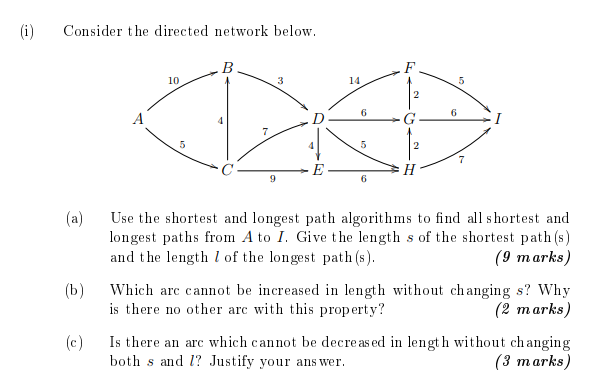
\includegraphics[width=\textwidth]{Network2014.png}
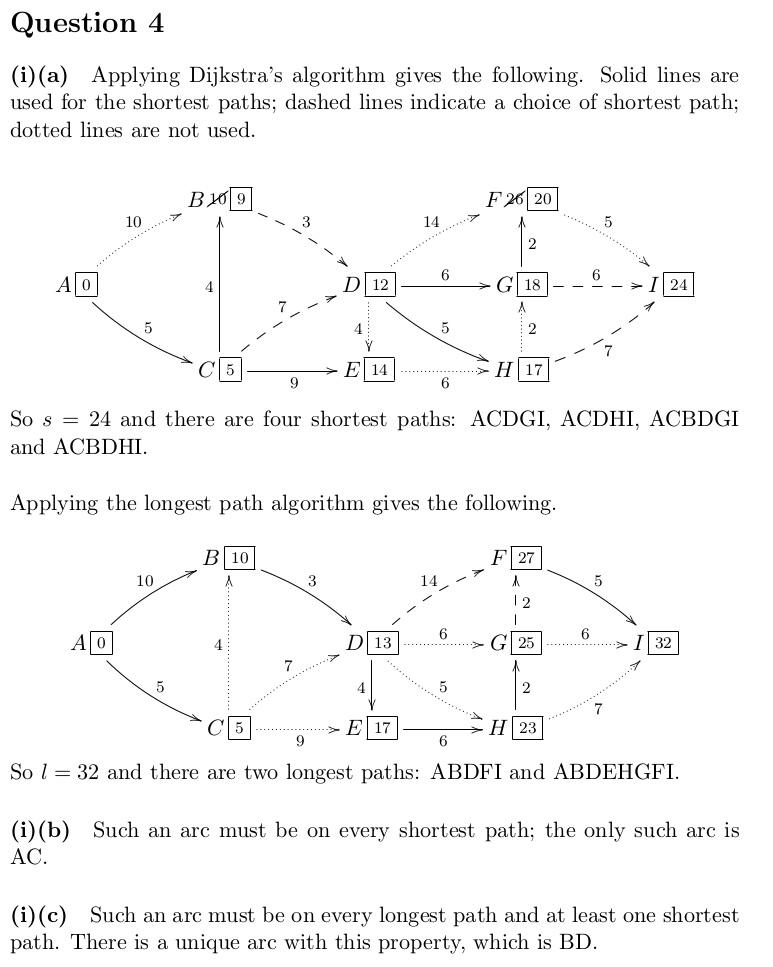
\includegraphics[width=.9\textwidth]{Network2014sol.png}

\subsubsection*{Comments:} This question was done well.  There are a couple of things you want to make sure are written/explained clearly, though, to make sure I don't miss them when marking 130 exams:
\begin{enumerate}
\item Write out all the longest/shortest paths when/where it asks you to; sometimes these were somewhere in your work but not restated clearly in the final answer
\item Make sure to explain your reasoning about which edges would length/shorten the shortest/longest path: ``Such an edge would have to be in \emph{all} longest paths -- those edges are ...''
\end{enumerate}

\section*{Question 3}
Find the Pr\"ufer code of the following tree:
\begin{center}
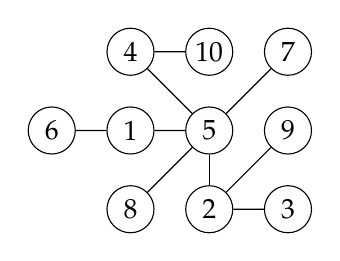
\begin{tikzpicture}
\tikzstyle{vertex}=[circle, draw, minimum size=17pt, inner sep=0pt]
\node[vertex] (1) at (0,1) {1};
\node[vertex] (2) at (1,0) {2};
\node[vertex] (3) at (2,0) {3};
\node[vertex] (4) at (0,2) {4};
\node[vertex] (5) at (1,1) {5};
\node[vertex] (6) at (-1,1) {6};
\node[vertex] (7) at (2,2) {7};
\node[vertex] (8) at (0,0) {8};
\node[vertex] (9) at (2,1) {9};
\node[vertex] (10) at (1,2) {10};

\draw (6)--(1)--(5)--(8);
\draw (10)--(4)--(5)--(7);
\draw (9)--(2)--(3);
\draw (2)--(5);

  \end{tikzpicture}
\end{center}

\begin{proof}
First we make a table of the edges, by pruning: iteratively deleting the leaf with the lowest label, and recording the leaf and the parent.  

$$\begin{array}{r|cccccccccc}
\text{Parent} & 2 & 1 & 5 & 5 & 5 &2 &5 &4 & 10 \\
\hline
\text{Leaf} & 3 & 6 & 1 & 7 & 8 & 9 & 2 & 5 & 4
\end{array}$$

The Pr\"ufer code is the top row, with the last entry removed, so 2,1,5,5,5,2,5,4.
\end{proof}
\subsubsection*{Comments}
The most common mistake was to include the last entry of the first row in the code, which is unnecessary: it can be figured out from all the previous entries!  The point of the Pr\"ufer code is not just to encode all labelled trees, but to do so without repetition or redunandant information, so that we have a bijection between codes and labelled trees, and hence a count of the labelled trees.





\end{document}
